% !TeX program = pdflatex
% AntiFLipper (v11, journal version) -- every result table, figure and in-text number is generated
% by make_results.py from the experiment outputs. Run it before compiling.
\documentclass[journal]{IEEEtran}

\usepackage{amsmath,amssymb,amsfonts}
\usepackage{graphicx}
\usepackage{booktabs}
\usepackage{pifont}
\usepackage{url}
\usepackage{tikz}
\usetikzlibrary{arrows.meta,positioning,fit,backgrounds,calc,shapes.geometric,shapes.symbols,shadows}
\usepackage[ruled,vlined,linesnumbered]{algorithm2e}
\usepackage{cite}

\newtheorem{proposition}{Proposition}
\newtheorem{corollary}{Corollary}
% generated by make_results.py -- do not edit
\newcommand{\headAcc}{72.0}
\newcommand{\headAccRaw}{71.0}
\newcommand{\headAccFLTrust}{69.2}
\newcommand{\headAccLFighter}{59.0}
\newcommand{\headAccFLAME}{56.9}
\newcommand{\headAccFedAvg}{44.2}
\newcommand{\headAccKrum}{60.8}
\newcommand{\headAccKrumStd}{15.8}
\newcommand{\headFPRFLTrust}{0.44}
\newcommand{\headFPRRaw}{0.08}
\newcommand{\headFPRcc}{0.25}
\newcommand{\headFPRcconly}{0.00}
\newcommand{\headRecallLFighter}{0.46}
\newcommand{\headRecallFLAME}{0.42}
\newcommand{\headASR}{3.2}
\newcommand{\headASRFedAvg}{32.8}
\newcommand{\headDet}{15}
\newcommand{\defMs}{30}
\newcommand{\defMsFedAvg}{34}
\newcommand{\defMsFLTrust}{352}
\newcommand{\rootMsFLTrust}{115}
\newcommand{\defMsFLAME}{1058}
\newcommand{\defMsKrum}{875}
\newcommand{\defMsLFighter}{42}
\newcommand{\evalOverhead}{6.8}
\newcommand{\cleanHonRaw}{18.3}
\newcommand{\cleanHon}{0.0}
\newcommand{\cleanHonBudget}{8.0}
\newcommand{\cleanHonCC}{17.0}
\newcommand{\cleanHonZthree}{17.7}
\newcommand{\cleanAccRaw}{16.3}
\newcommand{\cleanAcc}{54.3}
\newcommand{\cleanAccCROnly}{60.2}
\newcommand{\cleanAccBudget}{16.8}
\newcommand{\cleanAccMid}{66.5}
\newcommand{\cleanAccMidRaw}{40.7}
\newcommand{\cleanHonMidRaw}{16.0}
\newcommand{\skewAcc}{49.1}
\newcommand{\skewAccStd}{11.9}
\newcommand{\skewAccFedAvg}{43.8}
\newcommand{\skewAccFedAvgStd}{9.1}
\newcommand{\skewAccLFighter}{41.6}
\newcommand{\skewAccFLTrust}{39.3}
\newcommand{\skewAccRaw}{13.0}
\newcommand{\skewFPRRaw}{0.94}
\newcommand{\skewRecall}{0.96}
\newcommand{\skewRecallLFighter}{0.21}
\newcommand{\skewRecallFLTrust}{0.58}
\newcommand{\skewDet}{70}
\newcommand{\fakeRecallRaw}{0.67}
\newcommand{\fakeRecallCROnly}{0.62}
\newcommand{\fakeRecall}{1.00}
\newcommand{\fakeAcc}{72.0}
\newcommand{\ratioAccLow}{74.1}
\newcommand{\ratioAccFedAvgLow}{74.3}
\newcommand{\ratioAccThirty}{72.4}
\newcommand{\ratioAccFedAvgThirty}{61.0}
\newcommand{\ratioAccLFighterThirty}{64.9}
\newcommand{\ratioAccFLTrustThirty}{70.8}
\newcommand{\bnsafeHead}{57.8}
\newcommand{\mnistAcc}{98.7}
\newcommand{\iidAcc}{73.3}
\newcommand{\skewFull}{2/3}
\newcommand{\skewDetHits}{70}
\newcommand{\skewMissed}{1}
\newcommand{\fltrustNanRuns}{3}
\newcommand{\fltrustNanRounds}{6}
\newcommand{\bnsafeFPR}{0.33}
\newcommand{\cleanFinal}{46.1}
\newcommand{\cleanFinalMin}{10.3}
\newcommand{\cleanAccStd}{9.8}
\newcommand{\cleanAccCROnlyStd}{7.5}
\newcommand{\ccOverrideShare}{0.6}
\newcommand{\ratioFPRmax}{0.14}
\newcommand{\matchedOurs}{173}
\newcommand{\matchedFedAvg}{183}
\newcommand{\matchedFLTrust}{1269}
\newcommand{\matchedKrum}{4109}
\newcommand{\matchedFLAME}{3465}
\newcommand{\matchedLFighter}{214}
\newcommand{\matchedRaw}{176}
\newcommand{\nRuns}{396}
\newcommand{\ccHeadAcc}{72.2}
\newcommand{\ccHeadFPR}{0.00}
\newcommand{\ccSkewAcc}{44.6}
\newcommand{\ccSkewRecall}{0.04}
\newcommand{\ccCleanAcc}{55.2}
\newcommand{\fsFound}{1}
\newcommand{\fsTotal}{24}
\newcommand{\fedWCleanAcc}{59.7}
\newcommand{\fedWCleanStd}{10.5}
\newcommand{\fedWCleanFinal}{62.2}
\newcommand{\fedWSkewAcc}{44.8}
\newcommand{\fedWSkewStd}{9.2}
\newcommand{\fedWSkewASR}{21.4}
\newcommand{\pfAccFedAvgHalf}{71.9}
\newcommand{\pfAccFedAvgQuarter}{73.6}
\newcommand{\fedCleanAcc}{57.6}
\newcommand{\fedCleanStd}{9.4}
\newcommand{\fedCleanFinal}{51.9}
\newcommand{\fedCleanMid}{65.0}
\newcommand{\fedCleanHigh}{75.1}
\newcommand{\pfAccHalf}{71.3}
\newcommand{\pfAccQuarter}{72.1}
\newcommand{\pfDetHalf}{24}
\newcommand{\pfDetQuarter}{39}
\newcommand{\fakeDet}{13}
\newcommand{\fsAcc}{43.1}
\newcommand{\fsRecall}{0.04}
\newcommand{\fsRecallCR}{0.00}
\newcommand{\sizeLowMin}{143}
\newcommand{\sizeLowMax}{10{,}704}
\newcommand{\sizeHighMin}{1{,}244}
\newcommand{\sizeHighMax}{4{,}835}
\newcommand{\aucHighMin}{0.73}
\newcommand{\aucHighMax}{0.91}
\newcommand{\aucLowMin}{0.56}
\newcommand{\aucLowMax}{0.65}
\newcommand{\trajSeed}{19}
\newcommand{\fsAccFedAvg}{43.8}
\newcommand{\cleanWinsFedW}{0}
\newcommand{\skewWinsFedW}{2}
\newcommand{\skewWinsFed}{3}
\newcommand{\skewASR}{7.5}
\newcommand{\skewASRFedAvg}{18.7}
\newcommand{\skewASRBest}{3}
\newcommand{\pfASRHalf}{3.2}
\newcommand{\pfASRQuarter}{3.2}
\newcommand{\pfASRFedAvgHalf}{5.0}
\newcommand{\pfASRFedAvgQuarter}{3.7}
\newcommand{\fakeAucResHighMin}{0.70}
\newcommand{\fakeAucResHighMax}{0.73}
\newcommand{\fakeAucRawLowMin}{0.64}
\newcommand{\fakeAucRawLowMax}{0.73}
\newcommand{\fakeAucResLowMin}{0.46}
\newcommand{\fakeAucResLowMax}{0.58}
\newcommand{\sensAccMin}{98.4}
\newcommand{\sensAccMax}{98.8}
\newcommand{\sensFPRmax}{0.09}
\newcommand{\sensRecallMin}{1.00}


\begin{document}

\title{AntiFLipper: Label-Mix-Aware Accuracy Feedback Against Label-Flipping Attacks in Federated Learning}

\author{Aashnan Rahman, Abid Hasan, Sherajul Arifin, Faisal Haque Bappy, Tahrim Hossain, Tariqul Islam, Abu Raihan Mostofa Kamal, and Md. Azam Hossain
\thanks{A. Rahman, A. Hasan, A. R. M. Kamal and M. A. Hossain are with the Islamic University of Technology, Bangladesh. S. Arifin is with United International University, Bangladesh. F. H. Bappy, T. Hossain and T. Islam are with the University of Maryland, Baltimore County, United States.}}

\markboth{AntiFLipper: Label-Mix-Aware Accuracy Feedback Against Label Flipping}{Rahman \MakeLowercase{\textit{et al.}}}

\maketitle

\begin{abstract}
Label-flipping clients in federated learning (FL) run the unmodified training code on deliberately mislabeled data, so their updates resemble those of honest clients whose data are merely skewed. Accuracy feedback is a cheap countermeasure that needs no server data: each client reports how well the global model fits its local labels, and the server distrusts clients that report poorly. We show that this signal fails in two ways: it penalizes honest clients that hold hard classes, which under strong skew excluded \cleanHonRaw{} of 20 honest clients on average, and a flipper can report what an honest client would. We present AntiFLipper, which compares each report with the accuracy expected for the client's own label mix, computed from per-class counts (84 bytes per round), adds a last-layer consistency check taken from the update itself, and caps exclusions at the bound of the threat model. We analyze when this residual separates attackers and identify a self-inclusion bias that hides attackers holding most of a class. On CIFAR-10 with 40\% flippers under moderate skew, AntiFLipper reaches \headAcc\% accuracy against at most \headAccFLTrust\% for six baselines and excludes every attacker without a false positive, also under partial flips, report faking and half participation (\ppAcc\%). Under strong skew it excludes no honest client and, with attackers, attains the lowest attack success rate in every seed. Its server time is comparable to that of FedAvg. Report faking under strong skew remains unsolved (\fsFound{} of \fsTotal{} attackers detected), and our analysis explains why.
\end{abstract}

\begin{IEEEkeywords}
Federated learning, label flipping, data poisoning, data heterogeneity, malicious client detection, trust, robust aggregation.
\end{IEEEkeywords}

% =============================================================================
\section{Introduction}
\label{sec:intro}
% =============================================================================
\IEEEPARstart{F}{ederated} learning (FL) trains a shared model across many clients, such as phones, sensors or hospitals, without collecting their data~\cite{fedavg-pmlr-v54-mcmahan17a,kairouz2021advances}. The server sees only model updates and cannot check how they were produced, which exposes FL to data poisoning~\cite{lyu2020threats}. Its simplest form is \emph{label flipping}: a malicious client relabels its data, for instance by swapping pairs of classes, and trains as usual~\cite{biggio2011support,tolpegin2020data}. No change to the protocol or the training code is needed, so the attack is available to any participant that controls its own data pipeline, yet enough such clients steer the global model towards systematic misclassification of the targeted classes.

Detecting flippers is hard because honest clients differ as well. Each client holds its own mix of classes, and an unusual mix yields an unusual update. Defenses that inspect updates at the server, through robust statistics, distances or clustering~\cite{yin2018byzantine,NIPS2017_f4b9ec30,nguyen2022flame,jebreel2024lfighter}, are costly for large models and can mistake heterogeneous honest clients for attackers~\cite{li2023hscs,shen2024lfrppfl}. Defenses that score clients against clean data at the server~\cite{cao2020fltrust} need data that many deployments do not have, and whose distribution must match that of the clients.

A cheaper signal comes from the clients. If most clients are honest, the global model learns the true labels and fits a flipper's relabelled data poorly. Each client can evaluate the global model on its own data and report the result, and the server can lower the trust of clients that report poorly. This \emph{accuracy feedback} needs no server data and costs one forward pass per round~\cite{andreina2021baffle,jiang2023dataquality}. Used raw, however, it fails in two ways. First, an honest client that holds classes the model finds hard reports a low accuracy and is treated like an attacker. Under strong skew this cascades: excluding such clients removes their classes from training, which makes those classes harder still, and more clients fall below the threshold. Second, a report is only a claim, and a flipper can report what an honest client with the same data would report. Both problems grow with heterogeneity, exactly where update-based defenses struggle too.

This paper asks four questions:
\begin{itemize}
\item[\textbf{Q1}] Can accuracy feedback be corrected for label mix, so that skewed honest clients are no longer penalized, without losing its power to detect flippers?
\item[\textbf{Q2}] When does such a correction separate attackers from honest clients, and when does it fail?
\item[\textbf{Q3}] What must a defense observe besides reports to withstand attackers that fake them?
\item[\textbf{Q4}] How does the resulting defense compare with update-based and server-data-based defenses in accuracy, detection and cost, across heterogeneity, attacker shares, partial attacks and partial participation?
\end{itemize}

We answer them with \textbf{AntiFLipper}. The server asks not whether a client's accuracy is low, but whether it is lower than \emph{expected for the classes that client holds}. A second check inspects what the client actually sent, so that a convincing report alone is not enough to stay trusted. Our contributions are:
\begin{itemize}
\item \emph{A characterization of accuracy feedback.} Raw reports penalize label mix as well as poisoning (Prop.~\ref{prop:mix}); under strong skew this excluded \cleanHonRaw{} of 20 honest clients on average in our runs. No detector that reads only reports can identify a client that fakes them (Prop.~\ref{prop:faking}).
\item \emph{AntiFLipper.} It combines a \emph{class-conditional residual} computed from per-class report counts with a last-layer \emph{consistency check} of the update, keeps trust across rounds, and caps exclusions at the bound of the threat model. It needs no server data, sends 84 bytes per client and round, and its server time is comparable to that of FedAvg.
\item \emph{An analysis of the residual.} We show that it removes the label-mix penalty when per-class accuracies are known (Prop.~\ref{prop:cr}), and that its estimate has a self-inclusion bias that shrinks an attacker's residual in proportion to the attackers' share of its classes (Prop.~\ref{prop:bias}). The bias explains both the slower detection under strong skew and the case AntiFLipper does not solve.
\item \emph{An evaluation} on CIFAR-10 and MNIST against six defenses and two FedAvg variants (\nRuns{} training runs over three seeds), covering heterogeneity from mild to strong, 10--40\% attackers, partial flips, partial participation and report faking, with an ablation that attributes each result to a component, per-seed results where variance is high, a parameter study, and a matched cost benchmark.
\end{itemize}

The remainder is organized as follows. Section~\ref{sec:related} reviews related work and Section~\ref{sec:model} states the system and threat model. Section~\ref{sec:design} presents AntiFLipper and Section~\ref{sec:analysis} analyzes it. Sections~\ref{sec:setup} and~\ref{sec:results} describe the experiments and their results, Section~\ref{sec:discussion} discusses deployment and validity, and Section~\ref{sec:conclusion} concludes.

% =============================================================================
\section{Related Work}
\label{sec:related}
% =============================================================================
\subsection{Label flipping and data poisoning}
Label flipping was first studied as adversarial label noise in centralized learning, where flipping a small share of training labels degrades support vector machines substantially~\cite{biggio2011support}; optimized poisoning extends the idea to deep networks~\cite{munoz2017towards}. In FL, Tolpegin et al.~\cite{tolpegin2020data} showed that flipping the labels of one class sharply reduces accuracy on that class even with a minority of attackers, and that the damage grows with their share and with how early they join. Lavaur et al.~\cite{lavaur2024systematic} evaluate label flipping systematically across datasets and distributions and find that its effect depends strongly on heterogeneity. Shejwalkar et al.~\cite{shejwalkar2022backdrawingboard} argue that data poisoning is weak in production cross-device FL, where attackers are very few; with up to 40\% malicious clients, we model the stronger adversary of cross-silo settings or of deployments with many compromised devices. Crafted model updates~\cite{fang2020local,shejwalkar2021manipulating} and backdoors~\cite{bagdasaryan2020backdoor,wang2020attack} are different threats: they modify the training procedure or target specific inputs, whereas label flipping runs the honest code on wrong labels.

\subsection{Robust aggregation and anomaly detection}
Byzantine-robust aggregation bounds the influence of any minority of updates. Coordinate-wise Median and Trimmed Mean~\cite{yin2018byzantine} aggregate each coordinate robustly. Krum and Multi-Krum~\cite{NIPS2017_f4b9ec30} keep updates close to their nearest neighbors, and Bulyan~\cite{mhamdi2018hidden} combines both but needs $N\ge4f+3$ clients for $f$ attackers. These rules were designed for arbitrary (Byzantine~\cite{lamport1982byzantine}) updates and treat every outlier as suspicious. FoolsGold~\cite{fung2020limitations} down-weights clients whose update histories are similar, targeting sybils that pursue a common goal. FLAME~\cite{nguyen2022flame} clusters updates by cosine distance, clips them and adds noise, and CRFL~\cite{xie2021crfl} certifies robustness to backdoors through clipping, smoothing and parameter perturbation. All of these treat dissimilar updates as suspicious, yet under non-IID data honest updates are dissimilar too~\cite{li2020federated}, and their cost grows with the size of the full model.

\subsection{Defenses specific to label flipping}
Tolpegin et al.~\cite{tolpegin2020data} project the last-layer parameters of the attacked classes onto their principal components and cluster clients. LFighter~\cite{jebreel2024lfighter} clusters the gradients of the output neurons that changed most in a round, exploiting the observation that flipping concentrates on a few output classes. HSCS~\cite{li2023hscs} combines similarity with server-side data, and LFR-PPFL~\cite{shen2024lfrppfl} detects flippers from privacy-protected statistics. FLTrust~\cite{cao2020fltrust} trains on a small clean root dataset at the server each round and weights every client by the cosine similarity of its update with the server's, after normalizing magnitudes. These methods are effective when honest updates agree, but clustering separates heterogeneous honest clients as readily as attackers, and server data may be unavailable or unrepresentative.

\subsection{Client feedback and trust}
In BaFFLe~\cite{andreina2021baffle}, clients validate each new global model on their own data and vote on whether to accept it, which detects backdoors without server data. Other schemes estimate the quality of each client's labels~\cite{jiang2023dataquality,ovi2023confident}, derive trust from a guiding signal~\cite{li2025flgt}, align client distributions at two granularities~\cite{fedalign2026}, or add a detection pipeline~\cite{abroshan2025aitoprotect}. These approaches avoid server data but generally read a low score as evidence of poisoning, which conflates poisoning with label mix. They also rarely consider attackers that lie about their score. AntiFLipper belongs to this family. It differs in judging each report against what the client's own label mix predicts, in pairing reports with one cheap statistic of the update so that a faked report is not sufficient, and in bounding exclusions by the threat model. Table~\ref{tab:related} summarizes the differences.

\begin{table}[t]
\centering
\caption{Defenses against label flipping and poisoning: what they observe and need. $n$: participating clients, $W$: model parameters, $d_L$: last-layer parameters.}
\label{tab:related}
\scriptsize
\setlength{\tabcolsep}{2.5pt}
\begin{tabular}{@{}l l c c@{}}
\toprule
\textbf{Defense} & \textbf{Signal} & \textbf{Data}$^{*}$ & \textbf{Server cost} \\
\midrule
Median, TrMean~\cite{yin2018byzantine} & coordinate statistics & \ding{55} & $O(nW\log n)$ \\
Multi-Krum~\cite{NIPS2017_f4b9ec30} & pairwise distances & \ding{55} & $O(n^2W)$ \\
Bulyan~\cite{mhamdi2018hidden} & Krum + trimming & \ding{55} & $O(n^2W)$ \\
FoolsGold~\cite{fung2020limitations} & history similarity & \ding{55} & $O(n^2W)$ \\
FLAME~\cite{nguyen2022flame} & clustering, clipping & \ding{55} & $O(n^2W)$ \\
Tolpegin et al.~\cite{tolpegin2020data} & last-layer PCA & \ding{55} & $O(n^2 d_L)$ \\
LFighter~\cite{jebreel2024lfighter} & output-neuron clustering & \ding{55} & $O(n^2 d_L)$ \\
FLTrust~\cite{cao2020fltrust} & similarity to root update & \ding{51} & $O(nW)$ + training \\
BaFFLe~\cite{andreina2021baffle} & client validation votes & \ding{55} & $O(n)$ \\
\midrule
\textbf{AntiFLipper} & label-mix residual + CC & \ding{55} & $O(nK + n\,d_L)$ \\
\bottomrule
\end{tabular}
\\[2pt]\parbox{\linewidth}{\scriptsize $^{*}$Needs clean data at the server. Costs exclude the $O(nW)$ weighted average common to all methods.}
\end{table}

\subsection{Privacy of client statistics}
Per-class counts reveal a client's label histogram. Secure aggregation~\cite{bonawitz2017practical} lets the server learn only sums over clients, and LFR-PPFL~\cite{shen2024lfrppfl} protects detection statistics cryptographically. Section~\ref{sec:privacy} shows that AntiFLipper needs only pooled per-class sums and one scalar per client, so it is compatible with secure aggregation.

% =============================================================================
\section{System and Threat Model}
\label{sec:model}
% =============================================================================
\begin{table}[t]
\centering
\caption{Notation.}
\label{tab:notation}
\footnotesize
\setlength{\tabcolsep}{4pt}
\begin{tabular}{@{}ll@{}}
\toprule
\textbf{Symbol} & \textbf{Meaning} \\
\midrule
$N,\ T,\ K$ & clients, rounds, classes \\
$D_j,\ n_{jk},\ \pi_{jk}$ & client data, class-$k$ samples, label mix $n_{jk}/|D_j|$ \\
$\alpha_D$ & Dirichlet concentration of the data split \\
$M_t,\ m_{j,t}$ & global model, client model after local training \\
$S_t,\ \beta,\ n_t$ & sampled clients, excluded clients, active clients \\
$a_j,\ c_{jk}$ & reported accuracy, class-$k$ correct predictions \\
$\hat A_k,\ r_j$ & pooled class-$k$ accuracy, class-conditional residual \\
$\tau_j,\ \eta$ & trust, trust step size \\
$\delta_j,\ \tilde\delta,\ s_j$ & last-layer update, its median, cosine similarity \\
$z,\ \rho,\ c_{\max},\ g,\ b$ & CC cut-off, trust threshold, flag limit, warm-up, cap \\
$p,\ \pi(\cdot)$ & malicious share, label permutation \\
$w_k$ & attackers' trust-weighted share of class-$k$ counts \\
\bottomrule
\end{tabular}
\end{table}

\textbf{System.} A server coordinates $N$ clients over $T$ rounds (notation in Table~\ref{tab:notation}). Client $j$ holds a dataset $D_j$ with labels in $\{1,\dots,K\}$ and label mix $\pi_{jk}=n_{jk}/|D_j|$. In round $t$, a set $S_t$ of clients sampled from those not excluded receives the global model $M_t$; unless stated otherwise $S_t$ contains all of them. Each sampled client trains $M_t$ for $E$ local epochs and returns the model $m_{j,t}$, together with a report: the accuracy $a_j$ of $M_t$ on its local labels, its per-class correct counts $\mathbf{c}_j$ and its per-class sample counts $\mathbf{n}_j$. The server keeps a trust value $\tau_j$ per client, normalized to sum to one over the $n_t$ active clients, and a set $\beta$ of excluded clients. The server is honest but curious: it follows the protocol and may try to learn about client data from what it receives (Section~\ref{sec:privacy}).

\textbf{Adversary.} The adversary controls a fraction $p\le 0.4$ of the clients, chosen before training and fixed. Staying below one half keeps coordinate-wise medians informative and matches the regime in which robust aggregation is meaningful at all. Malicious clients relabel their data with the fixed permutation $\pi$: $0{\leftrightarrow}1$, $2{\leftrightarrow}3$, \dots, $8{\leftrightarrow}9$, and run the honest training code; their goal is to make the global model predict $\pi(y)$ for inputs of class $y$, measured by the attack success rate. A \emph{full flip} relabels all of a client's samples in every round. A \emph{partial flip} relabels a given fraction, drawn afresh at random in each round, which weakens both the attack and the signal it leaves. Attackers report in one of two ways:
\begin{itemize}
\item \emph{Honest reporting:} statistics of $M_t$ on the labels the client trains on.
\item \emph{Report faking (adaptive):} statistics of $M_t$ on the client's \emph{original} labels, as an honest client with the same data would report. This attacker knows that reports are used and keeps its own clean labels for the purpose.
\end{itemize}
Attackers know the protocol but not the trust values or the other clients' reports, and they do not collude beyond sharing $\pi$. Crafted updates such as gradient scaling or backdoors~\cite{bagdasaryan2020backdoor,fang2020local} are the domain of Byzantine-robust aggregation, with which AntiFLipper can be combined (Section~\ref{sec:discussion}).

\textbf{Goals.} A defense should (i) keep accuracy close to that of training without attackers, (ii) exclude or neutralize attackers, (iii) exclude no honest client, also without attackers and under strong skew, (iv) need no server data, and (v) add little computation and communication.

% =============================================================================
\section{AntiFLipper}
\label{sec:design}
% =============================================================================
AntiFLipper turns the two failure modes of accuracy feedback into two signals: the class-conditional residual corrects each report for label mix (Q1), and the consistency check observes the update instead of the report (Q3). Trust, flags and a capped exclusion rule turn both into an aggregation decision. Fig.~\ref{fig:arch} shows one round, and Algorithm~\ref{alg:af} lists the server side.

\begin{figure}[t]
\centering
\resizebox{\columnwidth}{!}{% AntiFLipper overview (one round). Included by AntiFlipper_v10.tex.
% Needs: \usetikzlibrary{arrows.meta,positioning,fit,backgrounds,calc,shapes.geometric,shapes.symbols}
% Grid: client lanes at x = 1.0 / 2.5 / 4.0; module bars start at x = 0.45;
%       M2/M5 end at x = 5.9; M4 occupies x = 6.45..8.25; M6 spans 0.45..8.25.
\definecolor{repc}{RGB}{38,99,170}\definecolor{repf}{RGB}{226,236,250}
\definecolor{updc}{RGB}{204,110,20}\definecolor{updf}{RGB}{253,237,219}
\definecolor{okc}{RGB}{22,150,100}\definecolor{badc}{RGB}{214,48,49}
\definecolor{barf}{RGB}{222,222,222}
\begin{tikzpicture}[
  font=\sffamily\small, >={Stealth[length=5pt,width=4pt]}, line cap=round,
  bar/.style={rounded corners=5pt, fill=barf, minimum height=0.62cm, align=center, inner sep=2pt},
  tok/.style={circle, minimum size=0.62cm, inner sep=0pt, font=\sffamily\footnotesize\bfseries},
  dia/.style={diamond, aspect=1, minimum size=0.82cm, inner sep=0pt, rounded corners=3pt, font=\sffamily\footnotesize\bfseries},
  group/.style={draw=black!45, dotted, line width=0.7pt, rounded corners=6pt},
  lbl/.style={font=\sffamily\scriptsize, align=left, text=black!75, anchor=west},
  w/.style={line width=0.9pt},
]
% ---------------------------------------------------------------- lanes and fixed columns
\def\xa{1.0}\def\xb{2.5}\def\xc{4.0}
\def\xl{4.6}   % left edge of the side labels
\def\xm{7.35}  % centre of M4
\def\ybus{0.95}
% ---------------------------------------------------------------- server frame (label sits on the frame line)
\draw[dashed, line width=0.8pt, rounded corners=9pt, black!70] (0.15,1.3) rectangle (8.55,7.05);
\node[font=\sffamily\small\bfseries, fill=white, inner sep=3pt, anchor=west] at (0.4,7.05) {Server};
% ---------------------------------------------------------------- clients (device card with a local data store)
\foreach \x/\n/\name/\col in {\xa/a/Client 1/black, \xb/b/Client 2/black, \xc/c/Attacker/badc}{
  \node[draw=\col, line width=1.1pt, rounded corners=4pt, minimum width=1.32cm, minimum height=0.95cm, fill=white] (cl\n) at (\x,0) {};
  \begin{scope}[shift={(\x-0.36,0.04)}, \col, line width=0.7pt]
    \draw[fill=white] (-0.16,0.16) -- (-0.16,-0.14) arc[start angle=180, end angle=360, x radius=0.16, y radius=0.055] -- (0.16,0.16);
    \draw[fill=white] (0,0.16) ellipse[x radius=0.16, y radius=0.055];
    \draw[line width=0.5pt] (-0.16,0.01) arc[start angle=180, end angle=360, x radius=0.16, y radius=0.055];
  \end{scope}
  \node[font=\sffamily\scriptsize, text=\col] at (\x+0.2,0.06) {$m_j$};
  \node[font=\sffamily\tiny, text=\col] at (\x,-0.33) {\name};
}
\node[font=\sffamily\tiny, text=badc, align=center, anchor=west] at (\xc+0.72,0.0) {flips\\labels};
% ---------------------------------------------------------------- M1: received reports
\node[group, minimum width=3.9cm, minimum height=0.95cm] at (\xb,2.05) {};
\foreach \x/\n/\c in {\xa/a/repc, \xb/b/repc, \xc/c/badc}
  \node[tok, fill=repf, draw=\c, line width=1.1pt] (r\n) at (\x,2.05) {M1};
\node[lbl] at (\xl,2.05) {Per-class\\reports (84\,B)};
% ---------------------------------------------------------------- M2
\node[bar, minimum width=5.45cm] (m2) at (3.175,3.1) {\textbf{M2:} Class-conditional residual \ $r_j$};
% ---------------------------------------------------------------- M3: per-client trust
\node[group, minimum width=3.9cm, minimum height=1.15cm] at (\xb,4.15) {};
\node[dia, fill=okc, text=white] (ta) at (\xa,4.15) {M3};
\node[dia, fill=okc, text=white] (tb) at (\xb,4.15) {M3};
\node[dia, fill=white, draw=badc, line width=1.1pt, text=badc] (tc) at (\xc,4.15) {M3};
\node[lbl] at (\xl,4.15) {Trust\\update $\tau_j$};
% ---------------------------------------------------------------- M5, M6
\node[bar, minimum width=5.45cm] (m5) at (3.175,5.15) {\textbf{M5:} Flags \& capped exclusion};
\node[bar, minimum width=7.8cm]  (m6) at (4.35,6.2)  {\textbf{M6:} Trust-weighted aggregation \ $\sum_{j\notin\beta}\tau_j m_j$};
% ---------------------------------------------------------------- M4 (update path): box with three stacked parts
\node[rounded corners=5pt, fill=updf, draw=updc, line width=0.9pt, minimum width=1.8cm, minimum height=3.9cm] (m4) at (\xm,3.55) {};
\node[align=center, anchor=north, inner sep=0pt] at ($(m4.north)+(0,-0.18)$) {\textbf{M4:}\\Update\\consistency\\check};
\draw[updc!60, line width=0.5pt] ($(m4.center)+(-0.6,0.1)$) -- ($(m4.center)+(0.6,0.1)$);
\node[font=\footnotesize] at ($(m4.center)+(0,-0.5)$) {$\cos(\delta_j,\tilde\delta)$};
\node[font=\sffamily\scriptsize, align=center, text=black!75] at ($(m4.center)+(0,-1.3)$) {last layer\\vs.\ median};
% ---------------------------------------------------------------- update bus (orange), clients -> M4
\foreach \n in {a,b,c}
  \draw[w, updc] ($(cl\n.north)+(0.42,0)$) -- ($(cl\n.north)+(0.42,\ybus-0.475)$);
\draw[w, updc, ->] ($(\xa+0.42,\ybus)$) -- (\xm,\ybus) -- (m4.south);
\node[font=\sffamily\scriptsize, text=updc, anchor=north] at (6.3,\ybus-0.04) {updates $m_j$};
% ---------------------------------------------------------------- report arrows (blue), centred on each M1, bridging the bus
\foreach \n/\c in {a/repc, b/repc, c/badc}
  \draw[w, \c, ->, preaction={draw=white, line width=3.4pt, shorten <=2pt, shorten >=2pt}] (cl\n.north) -- (r\n.south);
% ---------------------------------------------------------------- vertical flow through the modules
\foreach \n/\c in {a/black, b/black, c/badc}{
  \draw[w, \c, ->] (r\n.north) -- (r\n.north |- m2.south);
  \draw[w, \c, ->] (t\n.south |- m2.north) -- (t\n.south);
  \draw[w, \c, ->] (t\n.north) -- (t\n.north |- m5.south);
}
\foreach \x in {\xa,\xb}
  \draw[w, ->] (\x,5.46) -- (\x,5.89);
\draw[w, badc, dashed] (\xc,5.46) -- (\xc,5.6);
\node[circle, fill=badc, text=white, inner sep=0.6pt, font=\sffamily\tiny\bfseries] at (\xc,5.69) {$\times$};
\node[font=\sffamily\scriptsize, text=badc, anchor=west] at (\xc+0.18,5.69) {excluded};
% ---------------------------------------------------------------- M4 outputs
\draw[w, updc, ->] (m4.west |- m5) -- node[above, font=\sffamily\scriptsize, text=updc] {flag} (m5.east);
\draw[w, updc, ->] (m4.north) -- (m4.north |- m6.south);
% ---------------------------------------------------------------- global model and broadcast
\node[cloud, cloud puffs=11, cloud puff arc=110, aspect=2.2, draw=black!75, line width=0.9pt, fill=white,
      minimum width=2.3cm, minimum height=0.95cm, font=\sffamily\footnotesize, align=center] (gm) at (4.35,7.95) {Global model\\$M_{t+1}$};
\draw[w, ->] (m6.north) -- (gm.south);
\draw[w, ->] (gm.west) -- (-0.45,7.95) -- (-0.45,-0.95) -- (\xc,-0.95) -- (clc.south);
\foreach \n in {a,b} \draw[w, ->] (cl\n.south |- 0,-0.95) -- (cl\n.south);
\node[font=\sffamily\scriptsize, rotate=90, anchor=south] at (-0.45,3.4) {broadcast to active clients};
\end{tikzpicture}
}
\caption{One round of AntiFLipper. Each client sends a short report (blue) and its model update (orange). The server scores reports against each client's label mix, checks updates against the median, and aggregates only trusted clients; an attacker (red) is excluded.}
\label{fig:arch}
\end{figure}

\subsection{M1: Client report}
Before training, client $j$ runs one forward pass of $M_t$ over $D_j$ and records its accuracy $a_j$ and, for every class $k$, the numbers $c_{jk}$ of correct predictions and $n_{jk}$ of samples. With 32-bit values the payload is $4+8K$ bytes, i.e., 84 bytes for $K{=}10$, negligible next to the model update. The report is computed on the model the client receives, before local training, so it measures how well the current global model fits the client's labels rather than how well the client fits its own data.

\subsection{M2: Class-conditional residual}
The server pools per-class accuracy over the sampled clients, weighted by trust, and compares each report with the accuracy expected for that client's label mix:
\begin{equation}
\hat A_k=\frac{\sum_{i\in S_t} \tau_i c_{ik}}{\sum_{i\in S_t} \tau_i n_{ik}},\qquad
r_j=a_j-\sum_k \pi_{jk}\hat A_k .
\label{eq:cr}
\end{equation}
Classes without trust-weighted samples, and classes the client does not hold, are skipped, and $\pi_j$ is renormalized over the remaining classes. An honest client with hard classes reports a low $a_j$ but also has a low expectation, so its residual stays near zero. A flipper fits its own labels poorly in every class it holds, so its residual is negative, provided that $\hat A_k$ is dominated by honest clients. Trust weighting serves this purpose: as flippers lose trust, their contribution to $\hat A_k$ shrinks. Because $\hat A_k$ includes the scored client's own counts, however, the condition can fail for classes held mostly by flippers; Section~\ref{sec:analysis} quantifies this.

\subsection{M3: Trust update}
With $\bar r$ the mean residual over the sampled clients, trust moves by the squared deviation and is renormalized over the active clients:
\begin{equation}
\tau_j \leftarrow \max\!\big(0,\ \tau_j + \operatorname{sgn}(r_j-\bar r)\,\eta\,(r_j-\bar r)^2\big).
\label{eq:trust}
\end{equation}
The quadratic form damps small fluctuations, which are common under heterogeneity, and reacts strongly to persistent gaps. Trust persists across rounds, also for clients that are not sampled, so evidence accumulates over every round in which a client takes part.

\subsection{M4: Update-consistency check}
Let $\delta_j$ be the change of the classification layer (weights and bias) of client $j$ and $\tilde\delta$ the coordinate-wise median of all $\delta_j$ in the round. The server computes $s_j=\cos(\delta_j,\tilde\delta)$ and the robust score
\begin{equation}
\zeta_j=\frac{s_j-\operatorname{med}(s)}{1.4826\,\mathrm{MAD}(s)+\epsilon},
\label{eq:cc}
\end{equation}
with $\epsilon{=}10^{-6}$ for the case that all similarities coincide; the factor 1.4826 makes the median absolute deviation a consistent estimate of the standard deviation under normality. A client with $\zeta_j<-z$ is \emph{inconsistent}: its residual is replaced by the round minimum before~(\ref{eq:trust}), so that a good report cannot offset a deviating update, and it is flagged in M5. The check uses only the last layer, where label flipping acts most directly (Section~\ref{sec:analysis}), which keeps its cost independent of the size of the feature extractor.

\subsection{M5: Flags and capped exclusion}
After $g$ warm-up rounds, a client is flagged when $n_t\tau_j<\rho$, i.e., its trust falls below a fixed share $\rho$ of the uniform weight $1/n_t$ over the active clients, or when M4 marks it inconsistent. A client with $c_{\max}$ flags in total is excluded. Exclusions are capped at $b=\lfloor0.4N\rfloor$, the bound of the threat model; when more clients qualify, those with the lowest trust go first and the others keep their flags. The counter tolerates transient deviations, which heterogeneous honest clients show early in training, and the cap guarantees that no sequence of false positives removes more clients than the adversary could control.

\subsection{M6: Aggregation}
The server aggregates the sampled, non-excluded clients with their trust as weights:
\begin{equation}
M_{t+1}=\frac{\sum_{j\in S_t\setminus\beta}\tau_j\,m_{j,t}}{\sum_{j\in S_t\setminus\beta}\tau_j}.
\label{eq:agg}
\end{equation}
Initial trust is uniform, so before any evidence AntiFLipper equals equal-weight FedAvg.

\begin{algorithm}[t]
\caption{AntiFLipper: server side of round $t$}
\label{alg:af}
\small
\KwIn{models $m_{j,t}$, reports $(a_j,\mathbf{c}_j,\mathbf{n}_j)$ for $j\in S_t$; trust $\tau$; flag counts $c$}
$\hat A_k\leftarrow\sum_i\tau_ic_{ik}\,/\sum_i\tau_in_{ik}$ \ for every $k$ with $\sum_i\tau_in_{ik}>0$\;
\lForEach{$j\in S_t$}{$r_j\leftarrow a_j-\sum_k \pi_{jk}\hat A_k$ \ over the classes defined above, $\pi_j$ renormalized}
$\tilde\delta\leftarrow$ coordinate-wise median of last-layer updates $\{\delta_j\}$\;
$s_j\leftarrow\cos(\delta_j,\tilde\delta)$; \ $I\leftarrow\{j:\ (s_j-\operatorname{med}(s))/(1.4826\,\mathrm{MAD}(s)+\epsilon)<-z\}$\;
\lForEach{$j\in I$}{$r_j\leftarrow\min_i r_i$}
update $\tau$ with~(\ref{eq:trust}) and normalize over $j\notin\beta$\;
\If{$t\ge g$}{
 \ForEach{$j\in S_t$}{\lIf{$n_t\tau_j<\rho$ \textbf{\upshape or} $j\in I$}{$c_j\leftarrow c_j+1$}}
 $Q\leftarrow\{j\notin\beta:\ c_j\ge c_{\max}\}$ sorted by increasing $\tau_j$\;
 add the first $\max(0,\,b-|\beta|)$ clients of $Q$ to $\beta$; normalize $\tau$\;
}
\Return $M_{t+1}$ by~(\ref{eq:agg})
\end{algorithm}

% =============================================================================
\section{Analysis}
\label{sec:analysis}
% =============================================================================
Let $A_k$ be the accuracy of $M_t$ on inputs of true class $k$, and $C_{kl}$ the rate at which it predicts class $l$ for such inputs, so $A_k=C_{kk}$. We assume that these rates do not depend on which client a sample comes from, i.e., that clients differ in label mix but not in the distribution of inputs within a class. We take expectations over the client's samples for a fixed $M_t$.

\subsection{Raw feedback and the class-conditional residual}

\begin{proposition}[Raw feedback penalizes label mix]\label{prop:mix}
For an honest client, $\mathbb{E}[a_j]=\sum_k\pi_{jk}A_k$, so its deviation from the population mean is $\sum_k(\pi_{jk}-\bar\pi_k)A_k$, where $\bar\pi_k$ is the population share of class $k$.
\end{proposition}
\emph{Proof.} Each class-$k$ sample is classified correctly with probability $A_k$, and a fraction $\pi_{jk}$ of the client's samples are of class $k$. The population mean is $\sum_k\bar\pi_kA_k$. \hfill$\square$

The deviation is negative whenever a client holds more than its share of hard classes. It vanishes under IID data ($\pi_{jk}=\bar\pi_k$) and grows when each client holds few classes. Raw feedback therefore mixes two effects, label mix and poisoning, and the first dominates under strong skew. Exclusion amplifies it: removing clients that hold a hard class lowers $A_k$ for that class in later rounds, which lowers the reports of the remaining holders of class $k$, the cascade we observe in Section~\ref{sec:res-honest}.

\begin{proposition}[Residual with exact per-class accuracies]\label{prop:cr}
If $\hat A_k=A_k$ for all $k$, an honest client has $\mathbb{E}[r_j]=0$ for every label mix, while an honestly reporting flipper has $\mathbb{E}[r_j]=-\sum_k\pi_{jk}\,\big(A_{\pi(k)}-C_{k\pi(k)}\big)$, where $\pi_{jk}$ is the share of its samples of true class $k$.
\end{proposition}
\emph{Proof.} The first claim follows from~(\ref{eq:cr}) and Prop.~\ref{prop:mix}. A flipper's samples of true class $k$ carry label $\pi(k)$; they are counted under $\pi(k)$ and are correct only when $M_t$ predicts $\pi(k)$, at rate $C_{k\pi(k)}$, whereas the expectation for label $\pi(k)$ uses $A_{\pi(k)}$. \hfill$\square$

For a model that has learned the true labels, $A_{\pi(k)}$ is high and $C_{k\pi(k)}$ is low, so the flipper's expected residual is strongly negative regardless of its label mix. The residual thus removes the label-mix term of Prop.~\ref{prop:mix} while keeping the poisoning term.

\subsection{Estimation bias}
In practice $\hat A_k$ is estimated from the reports of a round, flippers included. We model this with a generic per-class deficit: an honest client reports class-$k$ accuracy $A_k$, an attacker reports $A_k-\Delta_k$ with $\Delta_k\ge0$. For an honestly reporting flipper, $\Delta_k=A_k-C_{\pi(k)k}$ by Prop.~\ref{prop:cr}; for a faking attacker, $\Delta_k$ is the leakage discussed after Prop.~\ref{prop:faking}. Let $w_k$ be the attackers' share of the trust-weighted class-$k$ counts in the denominator of~(\ref{eq:cr}).

\begin{proposition}[Self-inclusion bias]\label{prop:bias}
Under this model, $\hat A_k=A_k-w_k\Delta_k$ in expectation, and
\begin{equation}
\mathbb{E}[r_j]=\begin{cases}\ \ \sum_k \pi_{jk}\,w_k\,\Delta_k & \text{for an honest client,}\\ -\sum_k \pi_{jk}\,(1-w_k)\,\Delta_k & \text{for an attacker.}\end{cases}
\label{eq:bias}
\end{equation}
\end{proposition}
\emph{Proof.} The pooled class-$k$ accuracy is the count-weighted mean of $A_k$ over honest and $A_k-\Delta_k$ over attacking counts, i.e., $A_k-w_k\Delta_k$. Substituting into~(\ref{eq:cr}) with $a_j=\sum_k\pi_{jk}A_k$ (honest) or $\sum_k\pi_{jk}(A_k-\Delta_k)$ (attacker) gives~(\ref{eq:bias}). \hfill$\square$

\begin{corollary}\label{cor:bias}
An attacker whose classes are held mostly by attackers ($w_k\to1$) has an expected residual near zero, the value of an honest client in classes without attackers. Its residual is also pulled towards zero by its own counts, which enter $w_k$.
\end{corollary}

Two consequences follow. First, an honest client and an attacker with the \emph{same} label mix are separated by $\sum_k\pi_{jk}\Delta_k$ regardless of $w_k$, so the bias does not matter under mild skew, where label mixes overlap. Under strong skew, label mixes rarely overlap, and attackers that hold classes few honest clients hold are hidden by their own reports. Second, trust weighting helps only after attackers have lost trust; until then $w_k$ equals their share of the raw counts. Leaving the scored client out of $\hat A_k$ removes the self-inclusion part, and a robust per-class estimate (e.g., a trust-weighted median over clients instead of a pooled mean) would bound the influence of attackers holding class $k$; neither removes the bias when several attackers share a class without honest holders. Section~\ref{sec:res-auc} measures the separation empirically.

\subsection{Report faking}

\begin{proposition}[Report faking defeats report-only detection]\label{prop:faking}
Let a flipper report the statistics of $M_t$ on its original labels, and let $M_t$ not depend on the labels it trains with. Then its report has the same distribution as that of an honest client with identically distributed data, and no detector that reads only reports can separate the two better than chance.
\end{proposition}
\emph{Proof.} The faked report is the same function of $(M_t,x,y)$ as an honest report, and by assumption $M_t$ carries no trace of the flipped labels. Any test on reports therefore has equal acceptance probability for both. \hfill$\square$

The assumption holds in the first round. Later, $M_t$ has been trained on the flipper's own flipped samples, so its accuracy on the flipper's inputs may be lower than on an honest client's inputs of the same class; this is the \emph{leakage} $\Delta_k$ of Prop.~\ref{prop:bias}, which a report-only detector may exploit but cannot rely on. A defense must therefore also observe what a client \emph{did}. Relabelling class $k$ as $\pi(k)$ pushes the classifier row of $\pi(k)$ towards the features of class $k$ and vice versa, which we expect to oppose the last-layer change of honest clients that hold the same classes. With $p<1/2$, every coordinate of $\tilde\delta$ lies between honest values, as the coordinate-wise median has breakdown point $1/2$~\cite{yin2018byzantine}. This bounds the reference but does not guarantee that flippers obtain lower similarity than honest clients, whose similarities also spread under heterogeneity. We therefore treat the separation of M4 as an empirical property, use a conservative cut-off ($z{=}3$), and measure its false-positive rate in every setting.

\subsection{Exclusion bound and convergence}
A client flagged in $c_{\max}$ rounds after warm-up is excluded at its $c_{\max}$-th flag unless the cap is reached. The cap keeps at least $N-\lfloor0.4N\rfloor$ clients, so no sequence of false positives can empty the federation, and if all attackers are excluded within the cap, aggregation proceeds over honest clients only. We do not claim a convergence guarantee: even with fixed membership the trust weights in~(\ref{eq:agg}) change over time, so standard FedAvg analyses~\cite{li2020convergence} do not apply directly. Once membership and trust stabilize, AntiFLipper is FedAvg with fixed, non-uniform weights over the remaining clients, a setting covered by those analyses with an objective reweighted by trust. We report trajectories instead (Figs.~\ref{fig:traj} and~\ref{fig:pp}).

\subsection{Complexity}
\label{sec:complexity}
The report adds one forward pass over $D_j$ to $E$ training epochs, roughly a fraction $1/(3E)$ of the client's computation, since a backward pass costs about twice a forward pass. On the server, M2 costs $O(n_tK)$ and M4 $O(n_t d_L)$ for a last layer of $d_L$ parameters (5{,}130 for ResNet-18 on CIFAR-10), plus $O(n_tW)$ for the weighted average that every method performs. Multi-Krum costs $O(n_t^2W)$ for a $W$-parameter model, FLAME clusters $n_t^2$ similarities in dimension $W$, and FLTrust trains on server data every round (Table~\ref{tab:related}).

\subsection{Privacy}
\label{sec:privacy}
Per-class counts reveal a client's label histogram, and over repeated rounds they reveal it exactly. The server, however, needs only the pooled sums $\sum_i\tau_ic_{ik}$ and $\sum_i\tau_in_{ik}$ in~(\ref{eq:cr}) and one residual per client. A privacy-preserving variant proceeds as follows: (i) the server broadcasts $\tau$; (ii) clients submit $\tau_i\mathbf{c}_i$ and $\tau_i\mathbf{n}_i$ through secure aggregation~\cite{bonawitz2017practical}, so the server learns only their sums and hence $\hat A$; (iii) the server broadcasts $\hat A$; (iv) each client computes $r_j$ locally and sends it. The server then sees one scalar per client per round, as with raw accuracy feedback, and the last-layer update it already receives. A client could misreport $r_j$ in this variant, but it can equally misreport $a_j$ in the plain one; the consistency check covers both. We have not implemented this variant, and secure aggregation adds communication rounds and costs that we do not measure.

% =============================================================================
\section{Experimental Setup}
\label{sec:setup}
% =============================================================================
\subsection{Data, models and partitions}
CIFAR-10~\cite{CIFAR-krizhevsky2009learning} is trained with ResNet-18~\cite{resnet-he2016deep} (11.2\,M parameters) over 20 clients and 100 rounds, and MNIST~\cite{MNIST-lecun1998gradient} with a CNN of 21.8\,k parameters over 100 clients and 200 rounds; IID and non-IID splits use the same number of clients. Non-IID splits divide the samples of each class among the clients in proportions drawn from $\mathrm{Dir}(\alpha_D)$~\cite{hsu2019measuring}, with $\alpha_D{=}1$ (moderate skew) unless stated otherwise, $\alpha_D{=}0.5$, and $\alpha_D{=}0.1$ for strong skew. Client datasets are therefore unequal in size as well as in label mix: on CIFAR-10 they range from \sizeHighMin{} to \sizeHighMax{} samples at $\alpha_D{=}1$ and from \sizeLowMin{} to \sizeLowMax{} at $\alpha_D{=}0.1$. Table~\ref{tab:hyper} lists all training parameters.

\begin{table}[t]
\centering
\caption{Training and defense parameters.}
\label{tab:hyper}
\footnotesize
\setlength{\tabcolsep}{4pt}
\begin{tabular}{@{}lcc@{}}
\toprule
& \textbf{CIFAR-10} & \textbf{MNIST} \\
\midrule
Model (parameters) & ResNet-18 (11.2\,M) & CNN (21.8\,k) \\
Clients $N$, rounds $T$ & 20, 100 & 100, 200 \\
Local epochs $E$, batch size & 3, 32 & 3, 64 \\
Optimizer & \multicolumn{2}{c}{SGD, learning rate 0.01, momentum 0.9} \\
Weight decay & \multicolumn{2}{c}{$5\cdot10^{-4}$} \\
Participation & \multicolumn{2}{c}{all clients (half in Section~\ref{sec:res-partial})} \\
\midrule
AntiFLipper: trust & \multicolumn{2}{c}{$\eta{=}0.1$, $\rho{=}0.05$, $c_{\max}{=}6$, $g{=}2$} \\
AntiFLipper: CC, cap & \multicolumn{2}{c}{$z{=}3$, $b{=}\lfloor0.4N\rfloor$} \\
Multi-Krum & \multicolumn{2}{c}{$f=\lfloor pN\rfloor$} \\
FLTrust & \multicolumn{2}{c}{100 clean, class-balanced root samples} \\
\bottomrule
\end{tabular}
\end{table}

\subsection{Attacks}
By default 40\% of the clients perform a full flip and report honestly. This is the largest share our threat model allows and the hardest case, where undefended training and several baselines break down (Fig.~\ref{fig:ratio}). We also evaluate shares of 10--30\%; partial flips of 50\% and 25\%; partial participation, in which a random half of the active clients is sampled in every round; report faking at $\alpha_D{=}1$ and $0.1$; and runs without attackers at every level of skew, in which every exclusion is a false positive.

\subsection{Baselines and ablations}
We compare with FedAvg, coordinate-wise Median, Multi-Krum, FLAME, LFighter and FLTrust. FLTrust additionally receives its root set. Its reference implementation rescales all tensors including BatchNorm statistics, which produced non-finite losses in our ResNet-18 runs, so we also report a \emph{BN-safe} variant that rescales only trainable parameters; the partial-attack and participation experiments use this variant. Bulyan is not applicable, as $N{=}20$ and $f{=}8$ violate $N\ge4f+3$, and CRFL targets backdoors. FedAvg denotes equal client weights, as AntiFLipper's initial trust; under strong skew, where client sizes differ by orders of magnitude, we also run the original sample-weighted FedAvg~\cite{fedavg-pmlr-v54-mcmahan17a}. Ablations replace the residual with the raw report $a_j$, remove the consistency check (CC) or the cap, or use CC alone with uniform trust and the same $z$ and cap. All methods share partitions, attacker sets and seeds.

\subsection{Metrics}
Accuracy is measured on the full test set, and the attack success rate (ASR) is the share of test predictions equal to $\pi(y)$. Both are averaged over the last 10 rounds, since single rounds fluctuate by several points under strong skew. Precision, recall and false-positive rate (FPR) refer to the clients excluded, or given zero weight by baselines, in the final round. Under partial participation a baseline only judges the clients sampled in a round, so for baselines we report the share of sampled attackers (honest clients) given zero weight over the last 10 rounds. Results are means and standard deviations over three seeds (7, 19, 31), \nRuns{} training runs in total; the sensitivity study uses three separate held-out seeds. Server time covers all checks, trust updates and aggregation. We measure it during training on an RTX~3090 GPU, excluding rounds that overlapped other workloads, and in a matched CPU benchmark that gives every method the same 20 updates.

% =============================================================================
\section{Results}
\label{sec:results}
% =============================================================================
\begin{table*}[t]
\centering
\caption{Comparison with existing defenses under 40\% label-flipping clients (mean$\pm$std over three seeds).}
\label{tab:main}
\footnotesize
\setlength{\tabcolsep}{4.5pt}
\begin{tabular}{@{}l ccccc c cc@{}}
\toprule
& \multicolumn{5}{c}{\textbf{CIFAR-10, non-IID} ($\alpha_D{=}1$)} & \textbf{CIFAR-10} & \multicolumn{2}{c}{\textbf{MNIST}} \\
\cmidrule(lr){2-6}\cmidrule(lr){7-7}\cmidrule(lr){8-9}
\textbf{Method} & Acc.\,(\%)\,$\uparrow$ & ASR\,(\%)\,$\downarrow$ & Prec.\,$\uparrow$ & Rec.\,$\uparrow$ & FPR\,$\downarrow$ & IID Acc. & non-IID Acc. & IID Acc. \\
\midrule
FedAvg & 44.2{\scriptsize$\pm$0.5} & 32.8 & n/a & n/a & n/a & 42.1{\scriptsize$\pm$0.1} & 49.8{\scriptsize$\pm$0.3} & 49.6{\scriptsize$\pm$0.1} \\
Median & 57.9{\scriptsize$\pm$4.2} & 16.7 & n/a & n/a & n/a & 62.9{\scriptsize$\pm$1.4} & -- & -- \\
Multi-Krum & 60.8{\scriptsize$\pm$15.8} & 12.5 & 0.60 & 0.75 & 0.33 & 72.9{\scriptsize$\pm$0.3} & -- & -- \\
FLAME & 56.9{\scriptsize$\pm$7.7} & 17.7 & 0.49 & 0.42 & 0.17 & 71.1{\scriptsize$\pm$0.4} & -- & -- \\
LFighter & 59.0{\scriptsize$\pm$13.3} & 15.2 & 0.71 & 0.46 & 0.08 & 73.2{\scriptsize$\pm$0.3} & 98.5{\scriptsize$\pm$0.2} & \textbf{98.7}{\scriptsize$\pm$0.1} \\
FLTrust (reference)$^{\dagger}$ & 69.2{\scriptsize$\pm$1.1} & 5.2 & 0.60 & 0.92 & 0.44 & 63.1{\scriptsize$\pm$0.3} & 97.2{\scriptsize$\pm$0.1} & 97.5{\scriptsize$\pm$0.1} \\
FLTrust (BN-safe)$^{\dagger}$ & 57.8{\scriptsize$\pm$1.2} & 15.1 & 0.23 & 0.29 & 0.33 & 63.9{\scriptsize$\pm$2.3} & -- & -- \\
\midrule
\textbf{AntiFLipper} & \textbf{72.0}{\scriptsize$\pm$0.6} & \textbf{3.2} & \textbf{1.00} & \textbf{1.00} & \textbf{0.00} & \textbf{73.3}{\scriptsize$\pm$0.4} & \textbf{98.7}{\scriptsize$\pm$0.1} & \textbf{98.7}{\scriptsize$\pm$0.2} \\
\bottomrule
\end{tabular}
\\[2pt]\parbox{\linewidth}{\scriptsize $^{\dagger}$Uses a 100-sample clean root dataset at the server. Reference: rescales all tensors including BatchNorm statistics; BN-safe: trainable parameters only.}
\end{table*}

\begin{table*}[t]
\centering
\caption{Ablation on CIFAR-10: AntiFLipper with components removed (mean over three seeds).}
\label{tab:ablation}
\footnotesize
\setlength{\tabcolsep}{3.6pt}
\begin{tabular}{@{}l ccc cc ccc ccc cc@{}}
\toprule
& & & & \multicolumn{2}{c}{\textbf{40\% attack}} & \multicolumn{3}{c}{\textbf{40\% report faking}} & \multicolumn{3}{c}{\textbf{No attack}} & \multicolumn{2}{c}{\textbf{40\% attack}} \\
& & & & \multicolumn{2}{c}{$\alpha_D{=}1$} & \multicolumn{3}{c}{$\alpha_D{=}1$} & \multicolumn{3}{c}{$\alpha_D{=}0.1$} & \multicolumn{2}{c}{$\alpha_D{=}0.1$} \\
\cmidrule(lr){5-6}\cmidrule(lr){7-9}\cmidrule(lr){10-12}\cmidrule(lr){13-14}
\textbf{Variant} & CR & CC & Cap & Acc. & FPR & Acc. & Rec. & FPR & Acc.\,(last 10) & Acc.\,(final) & Excl.\,$\downarrow$ & Acc. & Rec. \\
\midrule
FedAvg & -- & -- & -- & 44.2 & n/a & 44.2 & n/a & n/a & 57.6{\scriptsize$\pm$9.4} & 51.9{\scriptsize$\pm$22.6} & n/a & 43.8 & n/a \\
FedAvg (sample-weighted) & -- & -- & -- & -- & n/a & -- & n/a & n/a & 59.7{\scriptsize$\pm$10.5} & 62.2{\scriptsize$\pm$7.2} & n/a & 44.8 & n/a \\
\midrule
Raw reports & \ding{55} & \ding{55} & \ding{55} & 71.0 & 0.08 & 72.4 & 0.67 & 0.08 & 16.3{\scriptsize$\pm$5.9} & 16.9{\scriptsize$\pm$5.7} & 18.3 & 13.0 & 0.88 \\
Raw reports + cap & \ding{55} & \ding{55} & \ding{51} & -- & -- & -- & -- & -- & 16.8{\scriptsize$\pm$6.4} & 16.7{\scriptsize$\pm$6.1} & 8.0 & 12.5 & 0.38 \\
Raw reports + CC & \ding{55} & \ding{51} & \ding{55} & 70.4 & 0.25 & 71.6 & 0.88 & 0.17 & 31.2{\scriptsize$\pm$15.2} & 31.4{\scriptsize$\pm$15.0} & 17.0 & 28.9 & \textbf{0.96} \\
CC only$^{\ddagger}$ & -- & \ding{51} & \ding{51} & \textbf{72.2} & \textbf{0.00} & 72.2 & \textbf{1.00} & \textbf{0.00} & 55.2{\scriptsize$\pm$7.8} & 52.0{\scriptsize$\pm$22.7} & 0.3 & 44.6 & 0.04 \\
CR + cap (no CC) & \ding{51} & \ding{55} & \ding{51} & 70.7 & \textbf{0.00} & \textbf{73.5} & 0.62 & \textbf{0.00} & \textbf{60.2}{\scriptsize$\pm$7.5} & \textbf{63.3}{\scriptsize$\pm$7.0} & 0.3 & \textbf{49.1} & \textbf{0.96} \\
\midrule
\textbf{AntiFLipper} & \ding{51} & \ding{51} & \ding{51} & 72.0 & \textbf{0.00} & 72.0 & \textbf{1.00} & \textbf{0.00} & 54.3{\scriptsize$\pm$9.8} & 46.1{\scriptsize$\pm$31.1} & \textbf{0.0} & \textbf{49.1} & \textbf{0.96} \\
\bottomrule
\end{tabular}
\\[2pt]\parbox{\linewidth}{\scriptsize Acc.: last-10-round mean unless marked. Excl.: honest clients excluded (of 20). FedAvg rows: no defense, for reference; the sample-weighted one weights clients by dataset size and was run only at $\alpha_D{=}0.1$. --: not run. CC uses $z{=}2.5$ in ``Raw reports + CC'' and $z{=}3$ elsewhere. $^{\ddagger}$Uniform trust; it ignores reports, so faking has no effect.}
\end{table*}


\subsection{Comparison with existing defenses}
\label{sec:res-main}
On CIFAR-10 non-IID with 40\% attackers (Table~\ref{tab:main}), AntiFLipper reaches \headAcc\% accuracy, the highest of all methods, and lowers the ASR from \headASRFedAvg\% under FedAvg to \headASR\%. In every seed it excludes all attackers, on average by round \headDet, and no honest client. The strongest baseline, the reference FLTrust, reaches \headAccFLTrust\% but needs server data, flags \headFPRFLTrust{} of the honest clients and produced non-finite losses in \fltrustNanRounds{} rounds across \fltrustNanRuns{} of its 3 runs; its BN-safe variant avoids these failures but reaches only \bnsafeHead\%. LFighter and FLAME find \headRecallLFighter{} and \headRecallFLAME{} of the attackers, and their accuracy, like that of Multi-Krum ($\pm$\headAccKrumStd), varies strongly across seeds: clustering succeeds in some seeds and splits honest clients in others. On CIFAR-10 IID and on MNIST, where heterogeneity is mild or absent, the strong methods lie within about a point of one another. The differences that matter appear with skewed data, which the following subsections examine.

\subsection{Ablation}
\label{sec:res-ablation}
Table~\ref{tab:ablation} attributes these results to components. In the main setting all feedback variants perform similarly, and CC alone, with the same $z$ and cap, is as accurate as AntiFLipper (\ccHeadAcc\%). The harder settings separate them. Raw reports fail without attackers under strong skew and against report faking; the cap alone limits the damage (\cleanHonBudget{} honest clients excluded instead of \cleanHonRaw) but does not prevent it. The residual prevents these exclusions and finds the attackers under strong skew, but misses fakers. CC alone catches every faker but finds only \ccSkewRecall{} of the attackers under strong skew, where its accuracy (\ccSkewAcc\%) matches undefended FedAvg. Each signal thus covers the failure of the other, and only the combination excludes no honest client without attackers, catches every faker under moderate skew and keeps the best recall under strong skew. The combination is not best everywhere: without attackers under strong skew, the residual alone is more accurate (\cleanAccCROnly\% against \cleanAcc\%).

\subsection{Honest clients under heterogeneity}
\label{sec:res-honest}
\begin{figure}[t]
\centering
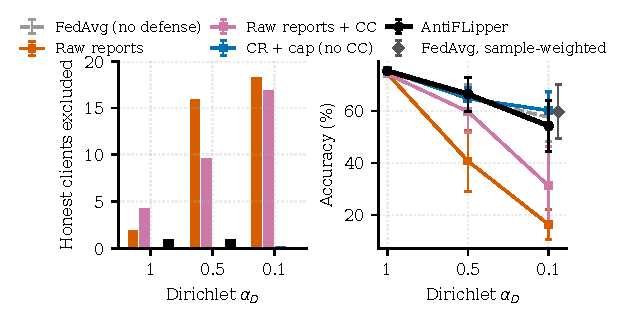
\includegraphics[width=\columnwidth]{fig/gen_heterogeneity.pdf}
\caption{No attackers: honest clients excluded (left) and accuracy (right) on CIFAR-10 as data become more skewed. Sample-weighted FedAvg was run at $\alpha_D{=}0.1$ only.}
\label{fig:het}
\end{figure}

\begin{figure}[t]
\centering
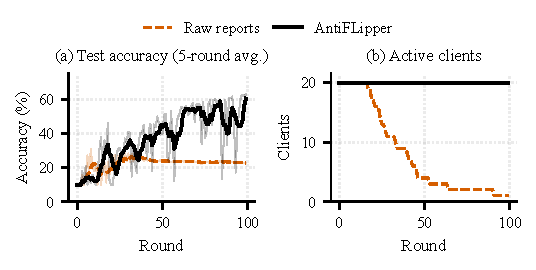
\includegraphics[width=\columnwidth]{fig/gen_trajectories.pdf}
\caption{One run without attackers at $\alpha_D{=}0.1$ (seed \trajSeed, the middle of our three seeds by number, not by outcome): raw reports exclude honest clients in a cascade; AntiFLipper excludes none.}
\label{fig:traj}
\end{figure}

Without attackers every exclusion is a false positive (Fig.~\ref{fig:het}). Raw reports exclude \cleanHonMidRaw{} of 20 honest clients at $\alpha_D{=}0.5$ and \cleanHonRaw{} at $\alpha_D{=}0.1$, where accuracy collapses to \cleanAccRaw\%. Fig.~\ref{fig:traj} shows the cascade predicted by Prop.~\ref{prop:mix}: exclusions accumulate round after round, and each one removes classes that make the next clients look worse. With the residual, exclusions stay near zero at every level of skew, and at $\alpha_D{=}0.5$ accuracy rises from \cleanAccMidRaw\% to \cleanAccMid\%.

The residual removes the penalty of raw feedback but does not make strongly skewed training more accurate than training without a defense. At $\alpha_D{=}0.1$, AntiFLipper averages \cleanAcc$\pm$\cleanAccStd\%, equal-weight FedAvg \fedCleanAcc$\pm$\fedCleanStd\% and sample-weighted FedAvg \fedWCleanAcc$\pm$\fedWCleanStd\%, which is ahead of AntiFLipper in each seed (Table~\ref{tab:seeds}). As CC marked only \ccOverrideShare\% of client-rounds and no honest client was excluded, the gap stems from the trust weights, which shift the trajectory considerably at this skew; even FedAvg ends at \fedCleanFinal\% on average in the final round, well below its last-10-round mean. Without attackers, AntiFLipper thus costs a few points of accuracy under strong skew, in exchange for the protection measured next.

\subsection{Attackers under strong skew}
\label{sec:res-skew}
\begin{table}[t]
\centering
\caption{Strong skew with attackers (CIFAR-10, $\alpha_D{=}0.1$, 40\% full flips, honest reports).}
\label{tab:skew}
\footnotesize
\setlength{\tabcolsep}{3.6pt}
\begin{tabular}{@{}l ccccc@{}}
\toprule
\textbf{Method} & Acc.\,(\%)\,$\uparrow$ & ASR\,$\downarrow$ & Rec. & FPR & All found \\
\midrule
FedAvg & 43.8{\scriptsize$\pm$9.1} & 18.7 & n/a & n/a & n/a \\
FedAvg (weighted) & 44.8{\scriptsize$\pm$9.2} & 21.4 & n/a & n/a & n/a \\
LFighter & 41.6{\scriptsize$\pm$11.5} & 19.0 & 0.21 & 0.28 & n/a \\
FLTrust$^{\dagger}$ & 39.3{\scriptsize$\pm$6.5} & 16.0 & 0.58 & 0.53 & n/a \\
\midrule
Raw reports & 13.0{\scriptsize$\pm$2.6} & 15.8 & 0.88 & 0.94 & 0/3 \\
\textbf{AntiFLipper} & \textbf{49.1}{\scriptsize$\pm$11.9} & \textbf{7.5} & \textbf{0.96} & \textbf{0.00} & 2/3 (70) \\
\bottomrule
\end{tabular}
\\[2pt]\parbox{\linewidth}{\scriptsize FedAvg: equal client weights; weighted: by dataset size, as in~\cite{fedavg-pmlr-v54-mcmahan17a}. All found: seeds in which every attacker was excluded (mean round).}
\end{table}

\begin{table}[t]
\centering
\caption{Per-seed results under strong skew (CIFAR-10, $\alpha_D{=}0.1$). Accuracy (\%) and, with attackers, ASR (\%).}
\label{tab:seeds}
\footnotesize
\setlength{\tabcolsep}{2.6pt}
\begin{tabular}{@{}l ccc cccccc@{}}
\toprule
& \multicolumn{3}{c}{\textbf{No attack}} & \multicolumn{6}{c}{\textbf{40\% attackers}} \\
\cmidrule(lr){2-4}\cmidrule(l){5-10}
\textbf{Seed} & 7 & 19 & 31 & \multicolumn{2}{c}{7} & \multicolumn{2}{c}{19} & \multicolumn{2}{c}{31} \\
\textbf{Method} & Acc. & Acc. & Acc. & Acc. & ASR & Acc. & ASR & Acc. & ASR \\
\midrule
FedAvg & 46.7 & 63.9 & 62.1 & 33.9 & 16.9 & 51.7 & 18.1 & 45.9 & 20.9 \\
FedAvg (weighted) & 48.1 & 62.7 & 68.4 & 40.4 & 21.6 & 55.4 & 13.2 & 38.7 & 29.5 \\
LFighter & -- & -- & -- & 28.5 & 16.9 & 50.2 & 17.2 & 46.0 & 22.9 \\
FLTrust & -- & -- & -- & 32.1 & 17.0 & 41.2 & 20.5 & 44.7 & 10.5 \\
Raw reports & -- & -- & -- & 15.6 & 14.0 & 13.1 & 23.3 & 10.3 & 10.0 \\
\textbf{AntiFLipper} & 45.1 & 53.1 & 64.5 & 35.8 & 9.0 & 59.0 & 7.4 & 52.4 & 6.3 \\
CR + cap (no CC) & 52.0 & 61.9 & 66.6 & -- & -- & -- & -- & -- & -- \\
\bottomrule
\end{tabular}
\\[2pt]\parbox{\linewidth}{\scriptsize Last-10-round means. --: not run in this setting.}
\end{table}

Table~\ref{tab:skew} adds 40\% attackers at $\alpha_D{=}0.1$. AntiFLipper reaches \skewAcc\%, against \skewAccFedAvg\% for FedAvg, \fedWSkewAcc\% for sample-weighted FedAvg, \skewAccLFighter\% for LFighter and \skewAccFLTrust\% for FLTrust. Accuracy varies widely across seeds for every method (Table~\ref{tab:seeds}), so we compare seed by seed: AntiFLipper beats FedAvg in \skewWinsFed{} of 3 seeds and sample-weighted FedAvg in \skewWinsFedW, and its ASR (\skewASR\%, against \skewASRFedAvg\% and \fedWSkewASR\%) is the lowest of all methods in each of the \skewASRBest{} seeds. Weighting by size raises the ASR, as large attackers gain influence. AntiFLipper finds \skewRecall{} of the attackers without excluding an honest client, whereas raw reports flag \skewFPRRaw{} of the honest clients and collapse to \skewAccRaw\%. Detection is slower and not always complete: all attackers were excluded in \skewFull{} seeds, by round \skewDetHits{} on average, and in the third seed \skewMissed{} attacker remained.

\subsection{Why detection is harder under strong skew}
\label{sec:res-auc}
\begin{table}[t]
\centering
\caption{Separation of attackers by their reports: AUC over the first 10 rounds, range over three seeds (0.5 = chance).}
\label{tab:auc}
\footnotesize
\setlength{\tabcolsep}{4pt}
\begin{tabular}{@{}cc l cc@{}}
\toprule
\textbf{Reports} & $\alpha_D$ & \textbf{Run} & Raw report $a_j$ & Residual $r_j$ \\
\midrule
Honest & 1 & AntiFLipper & 0.79--0.83 & 0.73--0.91 \\
Honest & 0.1 & AntiFLipper & 0.44--0.62 & 0.56--0.65 \\
\midrule
Faked & 1 & CR + cap & 0.54--0.70 & 0.70--0.73 \\
Faked & 0.1 & CR + cap & 0.64--0.73 & 0.46--0.58 \\
\bottomrule
\end{tabular}
\\[2pt]\parbox{\linewidth}{\scriptsize AUC: probability that a random attacker has a lower value than a random honest client, among active clients not marked by CC, averaged over rounds 0--9. Faking rows use the CR-only runs, where no client is marked by CC.}
\end{table}

To test Prop.~\ref{prop:bias}, we take the active clients that CC has not marked and compute, in each of the first ten rounds, the probability that a random attacker among them has a lower value than a random honest one (the AUC), then average over rounds. Table~\ref{tab:auc} reports the range over seeds. With honest reporting under moderate skew, both the raw report and the residual separate attackers well. Under strong skew the raw report is close to chance in some seeds, because label mix dominates it (Prop.~\ref{prop:mix}); the residual is better but far from the moderate-skew level, as Corollary~\ref{cor:bias} predicts when attackers hold classes with few honest holders. The two rows with faked reports are discussed in Section~\ref{sec:res-faking}.

\subsection{Partial flips and partial participation}
\label{sec:res-partial}
\begin{table*}[t]
\centering
\caption{Partial flips and partial participation (CIFAR-10 non-IID, $\alpha_D{=}1$, 40\% attackers, mean over three seeds).}
\label{tab:partial}
\footnotesize
\setlength{\tabcolsep}{3.4pt}
\begin{tabular}{@{}l cccc cccc cccc@{}}
\toprule
& \multicolumn{4}{c}{\textbf{Partial flip, 50\% of labels}} & \multicolumn{4}{c}{\textbf{Partial flip, 25\% of labels}} & \multicolumn{4}{c}{\textbf{Full flip, 50\% participation}} \\
\cmidrule(lr){2-5}\cmidrule(lr){6-9}\cmidrule(l){10-13}
\textbf{Method} & Acc.\,(\%) & ASR & Rec. & FPR & Acc.\,(\%) & ASR & Rec. & FPR & Acc.\,(\%) & ASR & Rec.$^{*}$ & FPR$^{*}$ \\
\midrule
FedAvg & \textbf{71.9} & 5.0 & n/a & n/a & \textbf{73.6} & 3.7 & n/a & n/a & 46.1{\scriptsize$\pm$3.0} & 30.6 & n/a & n/a \\
LFighter & 70.4 & 4.2 & 0.46 & 0.08 & 72.3 & 3.7 & 0.17 & 0.14 & 63.6{\scriptsize$\pm$6.5} & 10.0 & 0.84 & 0.13 \\
FLTrust (BN-safe)$^{\dagger}$ & 70.5 & 4.5 & 0.67 & 0.31 & 66.1 & 4.3 & 0.50 & 0.19 & 62.1{\scriptsize$\pm$2.6} & 11.1 & 0.50 & 0.15 \\
\midrule
\textbf{AntiFLipper} & 71.3 & \textbf{3.2} & \textbf{1.00} & \textbf{0.00} & 72.1 & \textbf{3.2} & \textbf{1.00} & \textbf{0.00} & \textbf{71.0}{\scriptsize$\pm$1.0} & \textbf{3.3} & \textbf{1.00} & \textbf{0.00} \\
\bottomrule
\end{tabular}
\\[2pt]\parbox{\linewidth}{\scriptsize Partial flip: share of each attacker's samples relabelled, a fresh random subset in every round; all clients take part. Participation: a random half of the active clients is sampled in every round. $^{\dagger}$BN-safe aggregation and a 100-sample clean root set. $^{*}$AntiFLipper: clients excluded in the final round. Baselines down-weight only the clients sampled in a round, so for them we report the share of sampled attackers (honest clients) given zero weight over the last 10 rounds.}
\end{table*}

\begin{figure}[t]
\centering
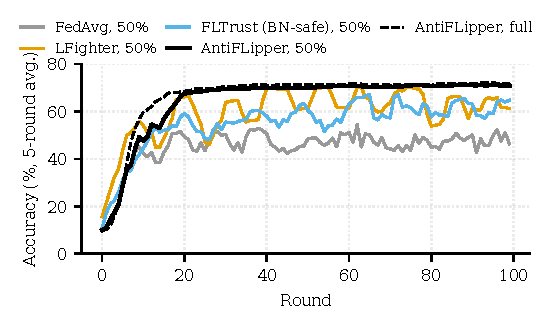
\includegraphics[width=\columnwidth]{fig/gen_participation.pdf}
\caption{Accuracy per round (mean over seeds, 5-round moving average) with half of the clients sampled in every round; AntiFLipper with full participation dashed for reference (CIFAR-10, $\alpha_D{=}1$, 40\% attackers).}
\label{fig:pp}
\end{figure}

\textbf{Partial flips.} An attacker that flips only part of its labels reports a higher accuracy and moves the model less. At both tested fractions AntiFLipper still excludes every attacker without false positives, by round \pfDetHalf{} at 50\% and \pfDetQuarter{} at 25\% (Table~\ref{tab:partial}). LFighter finds only \pfRecLFighterHalf{} and \pfRecLFighterQuarter{} of the attackers and the BN-safe FLTrust \pfRecFLTrustHalf{} and \pfRecFLTrustQuarter, both with false positives (FPR up to \pfFPRLFighterMax{} and \pfFPRFLTrustMax{} in single runs). These attacks are weak, however: FedAvg still reaches \pfAccFedAvgHalf\% and \pfAccFedAvgQuarter\%, close to its \fedCleanHigh\% without attackers and slightly above AntiFLipper (\pfAccHalf\% and \pfAccQuarter\%), which loses the correctly labelled part of the excluded clients' data while lowering the ASR from \pfASRFedAvgHalf\% to \pfASRHalf\% at 50\%. FLTrust was unstable in one run at 25\% (\pfAccFLTrustQuarterMin\%). Partial flips thus show that detection survives a weaker signal, not that it improves accuracy; a deployment that values the correctly labelled part of a partial flipper's data could down-weight instead of exclude.

\textbf{Partial participation.} In cross-device FL only part of the clients take part in a round. With a random half of the active clients sampled in every round (Table~\ref{tab:partial}, right; Fig.~\ref{fig:pp}), AntiFLipper reaches \ppAcc$\pm$\ppAccStd\%, close to its \headAcc\% with full participation, and again excludes every attacker without false positives in \ppFull{} seeds. Detection is slower (round \ppDet{} on average instead of \headDet), because each client collects flags only in the rounds in which it is sampled, which in turn delays the point at which the curve in Fig.~\ref{fig:pp} reaches that of full participation. LFighter reaches \ppAccLFighter$\pm$\ppAccLFighterStd\%, the BN-safe FLTrust \ppAccFLTrust\% and FedAvg \ppAccFedAvg\%, with ASRs of \ppASRLFighter\%, \ppASRFLTrust\% and \ppASRFedAvg\% against \ppASR\% for AntiFLipper. Baselines judge each round anew and give zero weight to \ppRecallLFighter{} (LFighter) and \ppRecallFLTrust{} (FLTrust) of the sampled attackers, but also to \ppFPRLFighter{} and \ppFPRFLTrust{} of the sampled honest clients. Trust that persists across rounds lets AntiFLipper combine evidence from every round in which a client took part, and once an attacker is excluded it can no longer be sampled.

\subsection{Report faking}
\label{sec:res-faking}
\begin{table}[t]
\centering
\caption{Attackers that try to stay hidden (CIFAR-10, 40\% attackers).}
\label{tab:adaptive}
\footnotesize
\setlength{\tabcolsep}{2.4pt}
\begin{tabular}{@{}l c cc ccccc@{}}
\toprule
& & \multicolumn{2}{c}{\textbf{FedAvg}} & \multicolumn{5}{c}{\textbf{AntiFLipper}} \\
\cmidrule(lr){3-4}\cmidrule(l){5-9}
\textbf{Attack} & $\alpha_D$ & Acc. & ASR & Acc.\,(\%) & ASR & Rec. & FPR & Found \\
\midrule
Full flip & 1 & 44.2 & 32.8 & 72.0{\scriptsize$\pm$0.6} & 3.2 & 1.00 & 0.00 & 3/3 (15) \\
\midrule
Partial, 50\% & 1 & 71.9 & 5.0 & 71.3{\scriptsize$\pm$0.4} & 3.2 & 1.00 & 0.00 & 3/3 (24) \\
Partial, 25\% & 1 & 73.6 & 3.7 & 72.1{\scriptsize$\pm$0.5} & 3.2 & 1.00 & 0.00 & 3/3 (39) \\
\midrule
Faking & 1 & 44.2 & 32.8 & 72.0{\scriptsize$\pm$0.3} & 3.3 & 1.00 & 0.00 & 3/3 (13) \\
Faking & 0.1 & 43.8 & 18.7 & 43.1{\scriptsize$\pm$9.8} & 17.2 & 0.04 & 0.06 & 0/3 \\
\quad CR only$^{*}$ & 0.1 & -- & -- & 44.5{\scriptsize$\pm$7.4} & 17.2 & 0.00 & 0.00 & 0/3 \\
\quad CC only$^{\ddagger}$ & 0.1 & -- & -- & 44.6{\scriptsize$\pm$7.6} & 19.0 & 0.04 & 0.03 & 0/3 \\
\bottomrule
\end{tabular}
\\[2pt]\parbox{\linewidth}{\scriptsize Partial: share of each attacker's samples relabelled, a fresh random subset in every round. FedAvg ignores reports, so its faking rows repeat the honest-reporting runs. $^{*}$Residual and cap, no consistency check. $^{\ddagger}$Consistency check and cap with uniform trust; it ignores reports, so its row is the honest-reporting run. Found: seeds in which every attacker was excluded (mean round).}
\end{table}

\textbf{Moderate skew.} Against attackers that fake their reports (Table~\ref{tab:adaptive}), AntiFLipper detects every faker, by round \fakeDet{} on average, with no false positives, and its accuracy (\fakeAcc\%) matches the honest-reporting case. Raw reports find \fakeRecallRaw{} of the fakers and the residual alone \fakeRecallCROnly. That report-only variants find any is the leakage noted after Prop.~\ref{prop:faking}: the residual of faked reports still ranks attackers below honest clients (AUC \fakeAucResHighMin--\fakeAucResHighMax, Table~\ref{tab:auc}), too weakly to exclude them all; the consistency check does.

\textbf{Strong skew.} Here faking succeeds: AntiFLipper finds \fsRecall{} of the attackers (\fsFound{} of \fsTotal{} over three seeds), and its accuracy (\fsAcc\%) is no better than that of FedAvg (\fsAccFedAvg\%). The logs show why. The raw faked reports still rank attackers below honest clients (AUC \fakeAucRawLowMin--\fakeAucRawLowMax), because the model has trained on the attackers' flipped samples, but the residual reduces this to \fakeAucResLowMin--\fakeAucResLowMax. This is Corollary~\ref{cor:bias} at work: under strong skew each class is concentrated on a few clients, so for classes held mostly by attackers, $\hat A_k$ consists largely of their own reports and absorbs their deficit. The correction that protects honest clients with unusual label mixes is the one that hides attackers with unusual label mixes. The consistency check alone finds \ccSkewRecall{} of the attackers, because honest last-layer updates already differ widely at this skew. This is the main open case.

\subsection{Share of malicious clients}
\label{sec:res-ratio}
\begin{figure}[t]
\centering
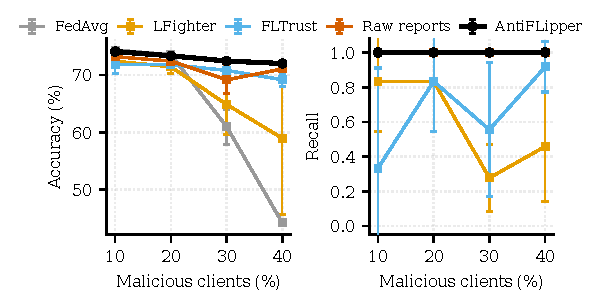
\includegraphics[width=\columnwidth]{fig/gen_ratio.pdf}
\caption{Accuracy and recall on CIFAR-10 non-IID ($\alpha_D{=}1$) versus the share of malicious clients.}
\label{fig:ratio}
\end{figure}
From 10\% to 40\% attackers (Fig.~\ref{fig:ratio}), AntiFLipper keeps a recall of 1.0 with an FPR of at most \ratioFPRmax{} (one or two honest clients in some seeds). At 10\% it matches undefended FedAvg (\ratioAccLow\% vs.\ \ratioAccFedAvgLow\%), so the defense costs nothing when the attack is weak. At 30\% it reaches \ratioAccThirty\%, while FedAvg drops to \ratioAccFedAvgThirty\%, LFighter to \ratioAccLFighterThirty\% and FLTrust to \ratioAccFLTrustThirty\%.

\subsection{Parameter sensitivity}
\label{sec:res-sens}
\begin{table}[t]
\centering
\caption{Parameter sensitivity of AntiFLipper (MNIST non-IID, held-out seeds).}
\label{tab:sensitivity}
\footnotesize
\setlength{\tabcolsep}{5pt}
\begin{tabular}{@{}l ccc@{}}
\toprule
& \multicolumn{2}{c}{\textbf{40\% attack}} & \textbf{No attack} \\
\cmidrule(lr){2-3}\cmidrule(lr){4-4}
\textbf{Setting} & Acc.\,(\%) & Rec. & FPR \\
\midrule
Default ($c_{\max}{=}6$, $z{=}3$) & 98.6 & 1.00 & \textbf{0.00} \\
\midrule
$c_{\max}=3$ & 98.6 & 1.00 & 0.02 \\
$c_{\max}=9$ & 98.6 & 1.00 & \textbf{0.00} \\
$z=2.5$ & 98.6 & 1.00 & 0.06 \\
$z=3.5$ & 98.6 & 1.00 & \textbf{0.00} \\
\bottomrule
\end{tabular}
\end{table}

We varied the flag limit $c_{\max}\in\{3,6,9\}$ and the cut-off $z\in\{2.5,3,3.5\}$ one at a time on MNIST non-IID with held-out seeds (Table~\ref{tab:sensitivity}). With 40\% attackers, accuracy stayed within \sensAccMin--\sensAccMax\% and recall at \sensRecallMin{} in every setting. Only the FPR without attackers reacted to the most aggressive settings ($c_{\max}{=}3$, $z{=}2.5$), reaching \sensFPRmax{} in a single run, which motivates the defaults. MNIST is an easy task, so this shows robustness to the parameters rather than to the data; the CIFAR-10 runs use the same defaults without tuning.

\subsection{Cost}
\label{sec:res-cost}
\begin{table}[t]
\centering
\caption{Cost per round on CIFAR-10 (ResNet-18, 20 clients).}
\label{tab:cost}
\footnotesize
\setlength{\tabcolsep}{3.2pt}
\begin{tabular}{@{}l ccccc@{}}
\toprule
& \textbf{Server} & \multicolumn{2}{c}{\textbf{Server time (ms)}} & \textbf{Client} & \textbf{Report} \\
\cmidrule(lr){3-4}
\textbf{Method} & \textbf{data} & matched & in training & \textbf{overhead} & \textbf{payload} \\
\midrule
FedAvg & \ding{55} & 183 & 34 & 0 & 0 \\
Multi-Krum & \ding{55} & 4109 & 875 & 0 & 0 \\
FLAME & \ding{55} & 3465 & 1058 & 0 & 0 \\
LFighter & \ding{55} & 214 & 42 & 0 & 0 \\
FLTrust$^{\dagger}$ & \ding{51} & 1269 & 352 + 115 & 0 & 0 \\
\midrule
\textbf{AntiFLipper} & \ding{55} & 173 & 30 & 6.8\% & 84\,B \\
\bottomrule
\end{tabular}
\\[2pt]\parbox{\linewidth}{\scriptsize Matched: identical 20 updates on one CPU (Intel i7-8700, 6 threads, PyTorch 2.8), mean of 5 timed iterations after one warm-up; standard deviation 8\,ms for AntiFLipper and 25\,ms for FedAvg. In training: measured per round on an RTX 3090 GPU; excluded clients are not averaged. FLTrust: aggregation + root training.}
\end{table}

In the matched benchmark (Table~\ref{tab:cost}), AntiFLipper's server work takes \matchedOurs\,ms, comparable to FedAvg (\matchedFedAvg\,ms), against \matchedFLTrust\,ms for FLTrust without root training, \matchedKrum\,ms for Multi-Krum and \matchedFLAME\,ms for FLAME. During training we observed \defMs\,ms per round, versus \defMsFedAvg\,ms for FedAvg; these times are not matched, because AntiFLipper averages fewer models once attackers are excluded. The client evaluation adds \evalOverhead\% to local training, below the $1/(3E)$ estimate of Section~\ref{sec:complexity}, as evaluation runs without gradients, and the 84-byte report is negligible next to the 44.7\,MB model update.

% =============================================================================
\section{Discussion}
\label{sec:discussion}
% =============================================================================
\textbf{When to use AntiFLipper.} The results suggest a simple guide. Under mild to moderate skew AntiFLipper is the most accurate method we tested, with complete and false-positive-free detection, also against partial flips, faked reports and partial participation, at the server cost of FedAvg and without server data. Under strong skew without attackers it costs a few points of accuracy, and with attackers it gives the lowest ASR but not reliably the highest accuracy. A deployment that expects strong skew and rare attacks may prefer sample-weighted FedAvg, possibly with AntiFLipper's detection as a monitor rather than as an aggregation rule.

\textbf{Why two signals.} The ablation shows that reports and updates fail in complementary situations. Reports fail when attackers lie, and updates fail when honest clients disagree. Neither failure is avoidable by tuning: Prop.~\ref{prop:faking} rules out report-only detection of faking, and under strong skew the spread of honest last-layer updates leaves CC alone with a recall of \ccSkewRecall. Combining them through a single trust value, with CC overriding the report rather than voting with it, lets each signal act where the other is blind.

\textbf{The residual's tension.} Report faking under strong skew exposes a tension in the residual itself. The residual helps honest clients precisely because it measures each client against a reference built from clients that hold the same classes; when those clients are attackers, the reference moves with them (Prop.~\ref{prop:bias}). A leave-one-out reference removes the scored client's own influence, and a robust per-class reference bounds the influence of the others. Both are cheap; neither helps when a class has no honest holders, where no statistic of reports can be expected to help and the update must carry the evidence.

\textbf{Combining with other defenses.} AntiFLipper changes only the weights and membership of aggregation. It can therefore precede a Byzantine-robust rule, which then operates on fewer and more homogeneous updates, or follow norm clipping against crafted updates. Combining its trust with sample weighting, to recover the accuracy of sample-weighted FedAvg under strong skew, is untested.

\textbf{Threats to validity.} Internally, baselines were run with our implementations under shared partitions; the reference FLTrust was unstable with BatchNorm, which we addressed with a BN-safe variant and report both. Last-10-round averages reduce but do not remove the noise of single rounds, and three seeds support means and standard deviations, not fine-grained significance claims; under strong skew we therefore report per-seed results. Externally, our experiments cover image classification with two datasets and models, one permutation attack, synchronous rounds and uniform client sampling at one rate; other domains, targeted single-class flips, colluding attackers and data-dependent dropout may behave differently.

% =============================================================================
\section{Limitations and Future Work}
\label{sec:limits}
% =============================================================================
AntiFLipper does not solve report faking under strong skew (\fsFound{} of \fsTotal{} attackers detected); a leave-one-out or robust per-class reference is the most direct next step, and an attacker that also aligns its last-layer update with the median could evade CC under moderate skew. Colluding attackers, which could coordinate their updates to move the median, were not evaluated. Under strong skew with honest reporting, detection was incomplete in one of three runs, and without attackers AntiFLipper is less accurate than undefended FedAvg. We give no convergence guarantee, and per-class counts reveal label histograms unless the secure-aggregation variant is deployed, which we have not implemented. Our experiments cover synchronous image classification on a single GPU server; partial participation was tested only at one rate with uniform sampling, and dropout that correlates with data, asynchronous updates, other domains such as text or tabular data, larger federations and edge hardware remain to be tested.

% =============================================================================
\section{Conclusion}
\label{sec:conclusion}
% =============================================================================
Accuracy feedback is a cheap, data-free signal against label flipping, but used raw it mistakes skewed honest clients for attackers and can be faked. AntiFLipper judges each report against the client's own label mix and checks the update itself, with trust that persists across rounds and exclusions bounded by the threat model. Under moderate skew it is more accurate than all six baselines, with complete, false-positive-free detection also against partial flips and faked reports and when only half of the clients take part in each round. Under strong skew it reduced the honest clients wrongly excluded from \cleanHonRaw{} of 20 to zero and, with attackers, gave the lowest ASR in every seed, at a server cost comparable to FedAvg. Our analysis shows that the residual's estimate is biased by the attackers' share of each class, which explains both the slower detection under strong skew and the open case of report faking there: the label-mix correction that protects honest clients also hides the attackers. Resolving this tension, through references that exclude the scored client or resist attackers that dominate a class, is the main direction for future work.

\bibliographystyle{IEEEtran}
\bibliography{IEEEabrv,bibliography_updated}
\end{document}
